%\subsection{}

In the previous section,  we defined the notion of
typical number of words in the support of a topic, or sig\_words, and
the notion of a typical number of topics in a document.  Clearly, if
both get very large one gets to a trivial topic model where each document
is generated by choosing words independently from a single probability
distribution.  

On the other hand if sig\_words and sig\_topics are small
each document should have relatively small support
compared with the corpus. Thus, in such cases we should
easily distinguish the data from the trivial topic model.

%% Here we derive an easy to compute quantity based on sig\_words,
%% sig\_topics, the total number of topics, and the corpus size to
%% predict when learning a topic model becomes difficult to distinguish
%% from the trival model.

%% Recall from the previous section, that LdaT had access included a
%% ``topic'' cheater method that knew the topic distributions while not
%% knowing anything about document topics (other than some of the words
%% in the document.)  The other algorithms were only given the actual
%% documents.

%% We wish to understand when knowing just the topic matrix is sufficient
%% and when our algorithm performs worse than the topic cheater.  We
%% compute a quantity that is reasonably predictive of both events.
%% Moreover, the point at which the algorithm performs poorly against the
%% cheater would perhaps be when the algorithm fails to learn the topics
%% well.  We examine this aspect later in this section.

We will proceed by showing that the probability of cooccurrence in
documents of two words $i$ and $j$ differs significantly from in the
trivial topic model. This can be represented as a matrix which
refer to as the co-occurence matrix.

The expected co-occurence matrix can, of course, be calculated
precisely from the topic and document distributions.  But we give
simple, even trivial, calculations that provide insight based on a
simplified topic model.

\subsection{A Uniform Topic Model.}

We proceed by calculating the difference in co-occurence matrices of a
corpus generated by a nontrivial topic model from the trivial topic
model.

Let $k$ be the total number of topics. Let $m$ be the vocabulary size. Let
$t$ be the number of topics in a document and assume that 
each word is chosen uniformly from these $t$ topics. Each topic is a
uniform distribution over $w$ words. 
%% In some sense, $t$ is a proxy for sig\_topics and
%% $w$ is a proxy for sig\_words. 
Let $l$ be the number of words in the document.

We examine word cooccurrences for $w_i$ and $w_j$: that is, the
probability that two words generated in a document are $w_i$ and
$w_j$.  Note that in a document of length $l$, there are ${l \choose
2}$ possible cooccurences between $w_i$ and $w_j$.

We compute the probability of a word cooccurrence for data from a
topic distribution versus  the trivial model with the working
vocabulary: the union of significant words in all topics which roughly has
size $v = \min(m,kw)$.

For two words from the same topic, a document contains their common
topic with probabiltiy $t/k$, and the probability that both words are
chosen is $(1/tw)^2$. Thus the probability of cooccurence from being
in the same topic is $\frac{t}{k} (1/tw)^2$.  We assume that the background
probability that the two words cooccur in the other case (or in the
case that there are no topics) is $1/v^2$.  \footnote{We note that it
is possible to set up topics so that the additional correlations one
recieves in one topic are exactly cancelled out by other topics.  This
setup corresponds to coding up a parity problem in the set of topics,
but it seems unlikely to arise in any reasonable topic model.  Still,
the ``rough'' calculations here fail. Indeed, we emphasize that the
arguments are heuristic.}

When the background co-occurrence is much smaller than the
topic cooccurrence the topic model should be easy to learn.  For
example, when $\frac{t}{k}{1/(tw)^2} >> 1/v^2$ or when $1 >>
(\frac{kw}{v})^2 \frac{t}{k}$, then we should have good
performance. In figure \ref{fig:ratio}, we plot this ratio against the
performance of the projector algorithm and see that things degrade as
this value increases.


We note that technically even under the weaker condition that $tw <
v$, an algorithm could information theoretically determine the topics
with enough data but the benefit over the baseline algorithm will be
small. 

\begin{figure}[t]
%     \begin{center}
                  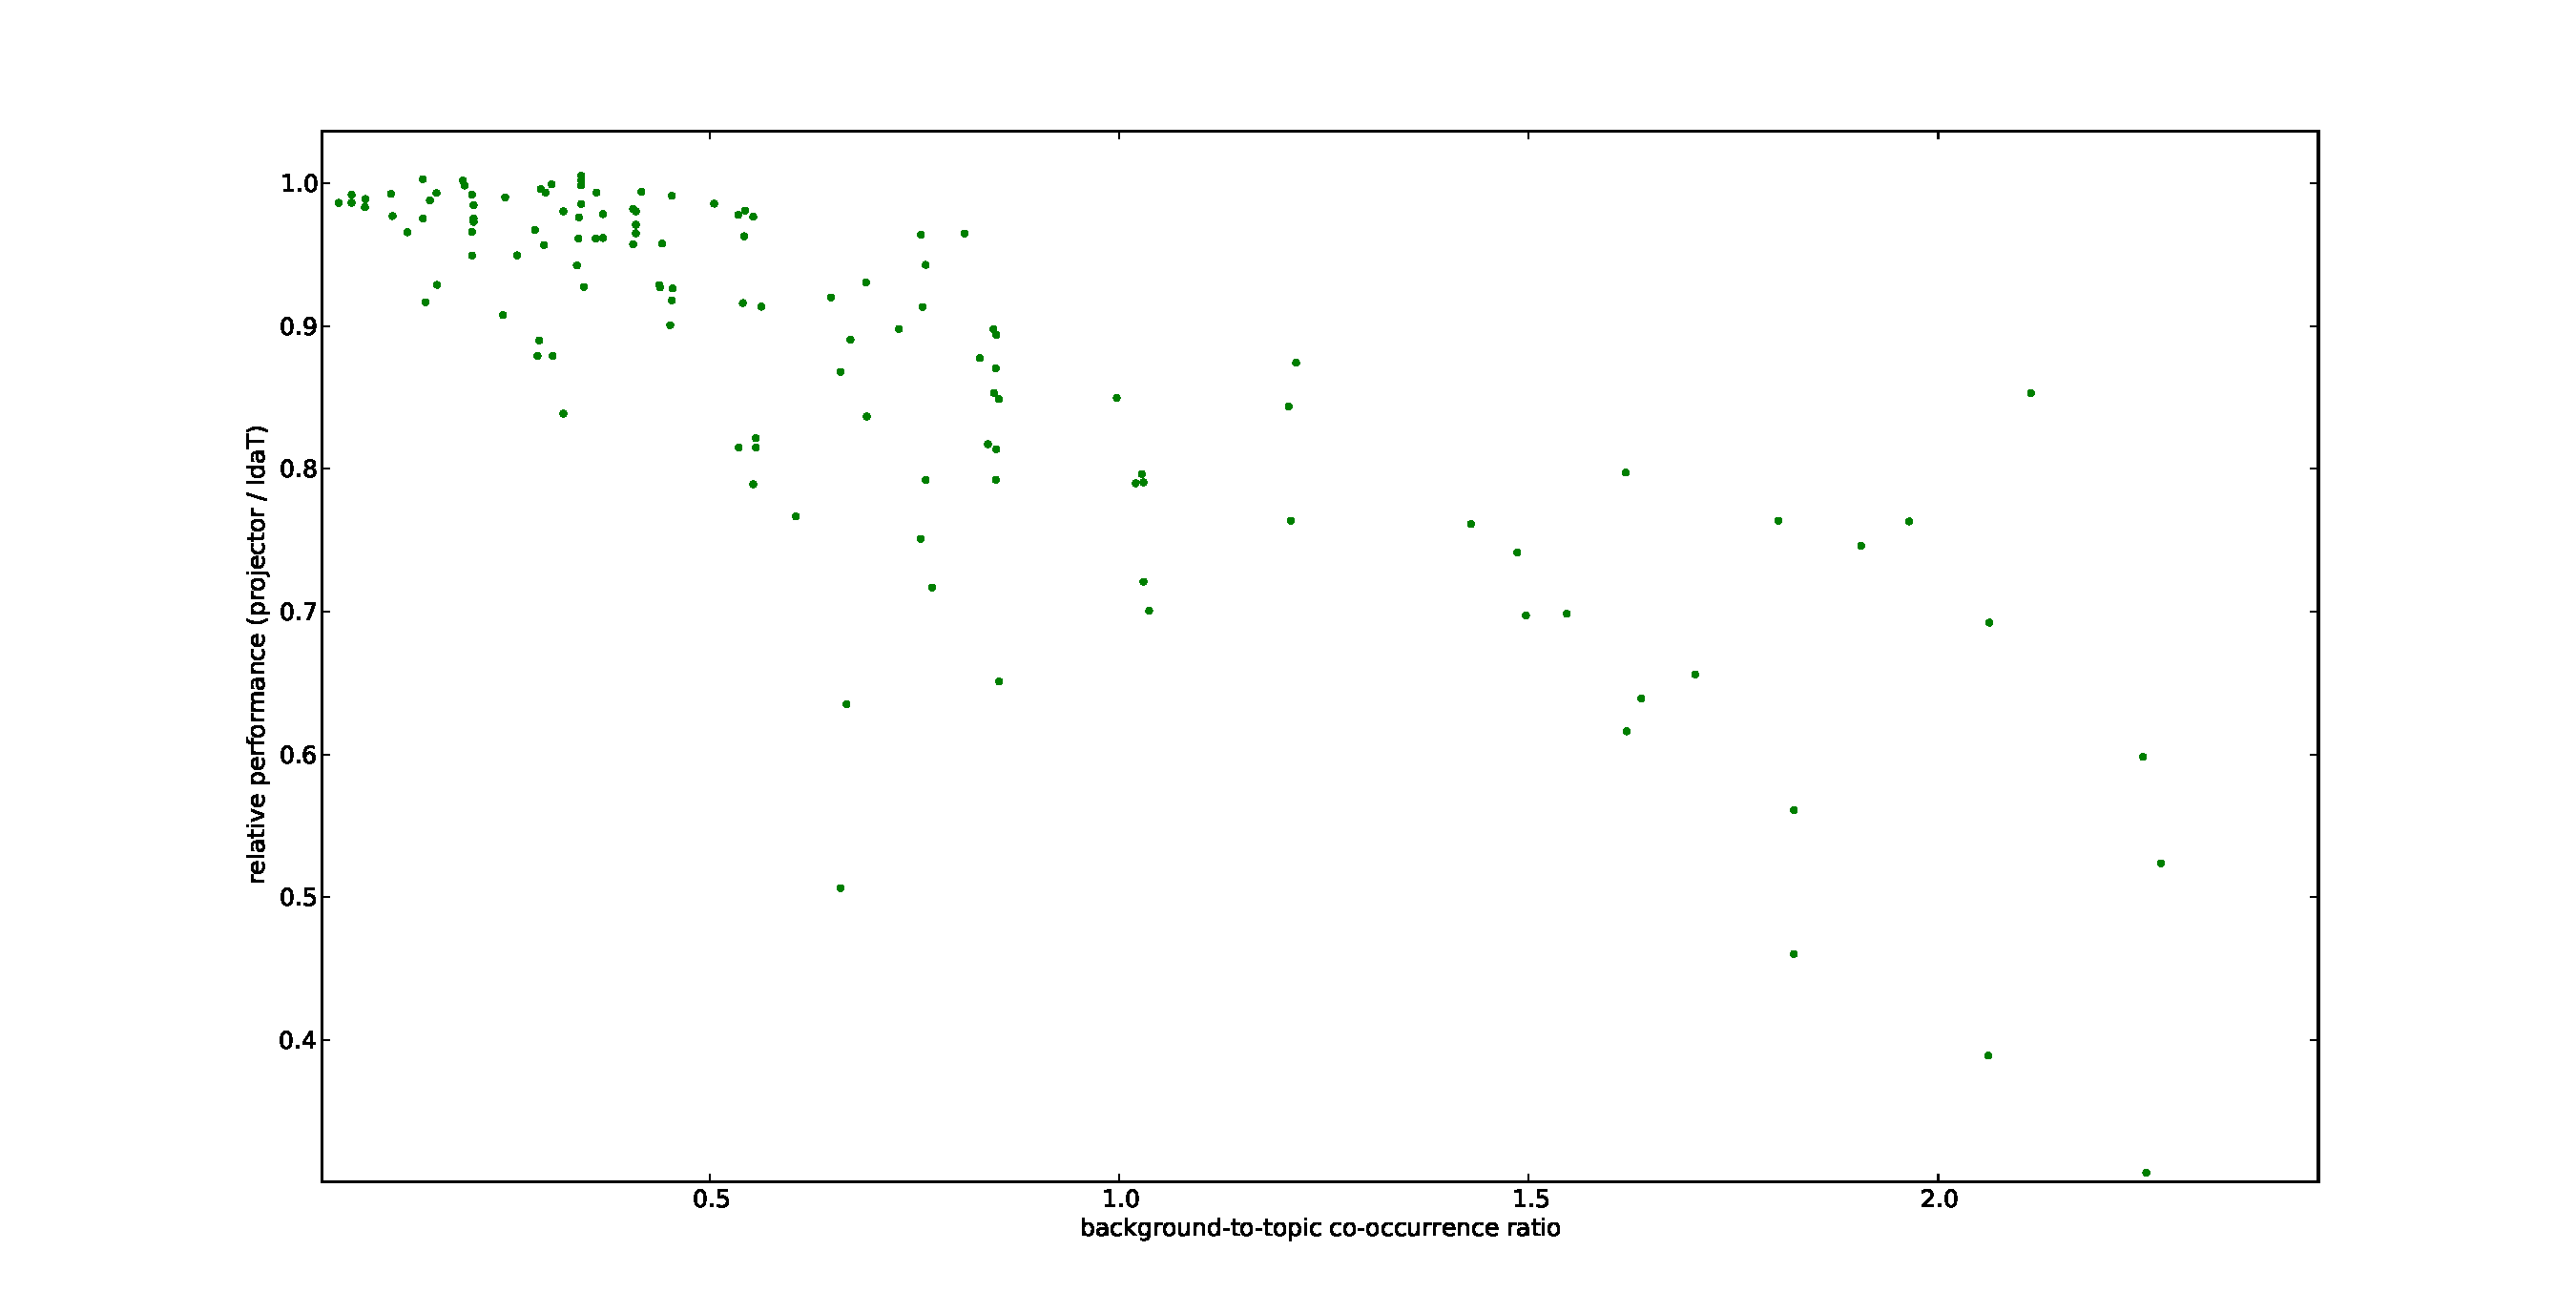
\includegraphics[width=0.58\textwidth]{projldaT-ratio.pdf}
%    \end{center}
    \caption{The performance of projector relative to LDAT falls off as the ratio of the background
to topic cooccurrences increases.
}
   \label{fig:ratio}
\end{figure}



\subsection{Dependence on document length and number.}


\begin{figure}
     \begin{center}

        \subfigure[]{
            \label{fig:a}
            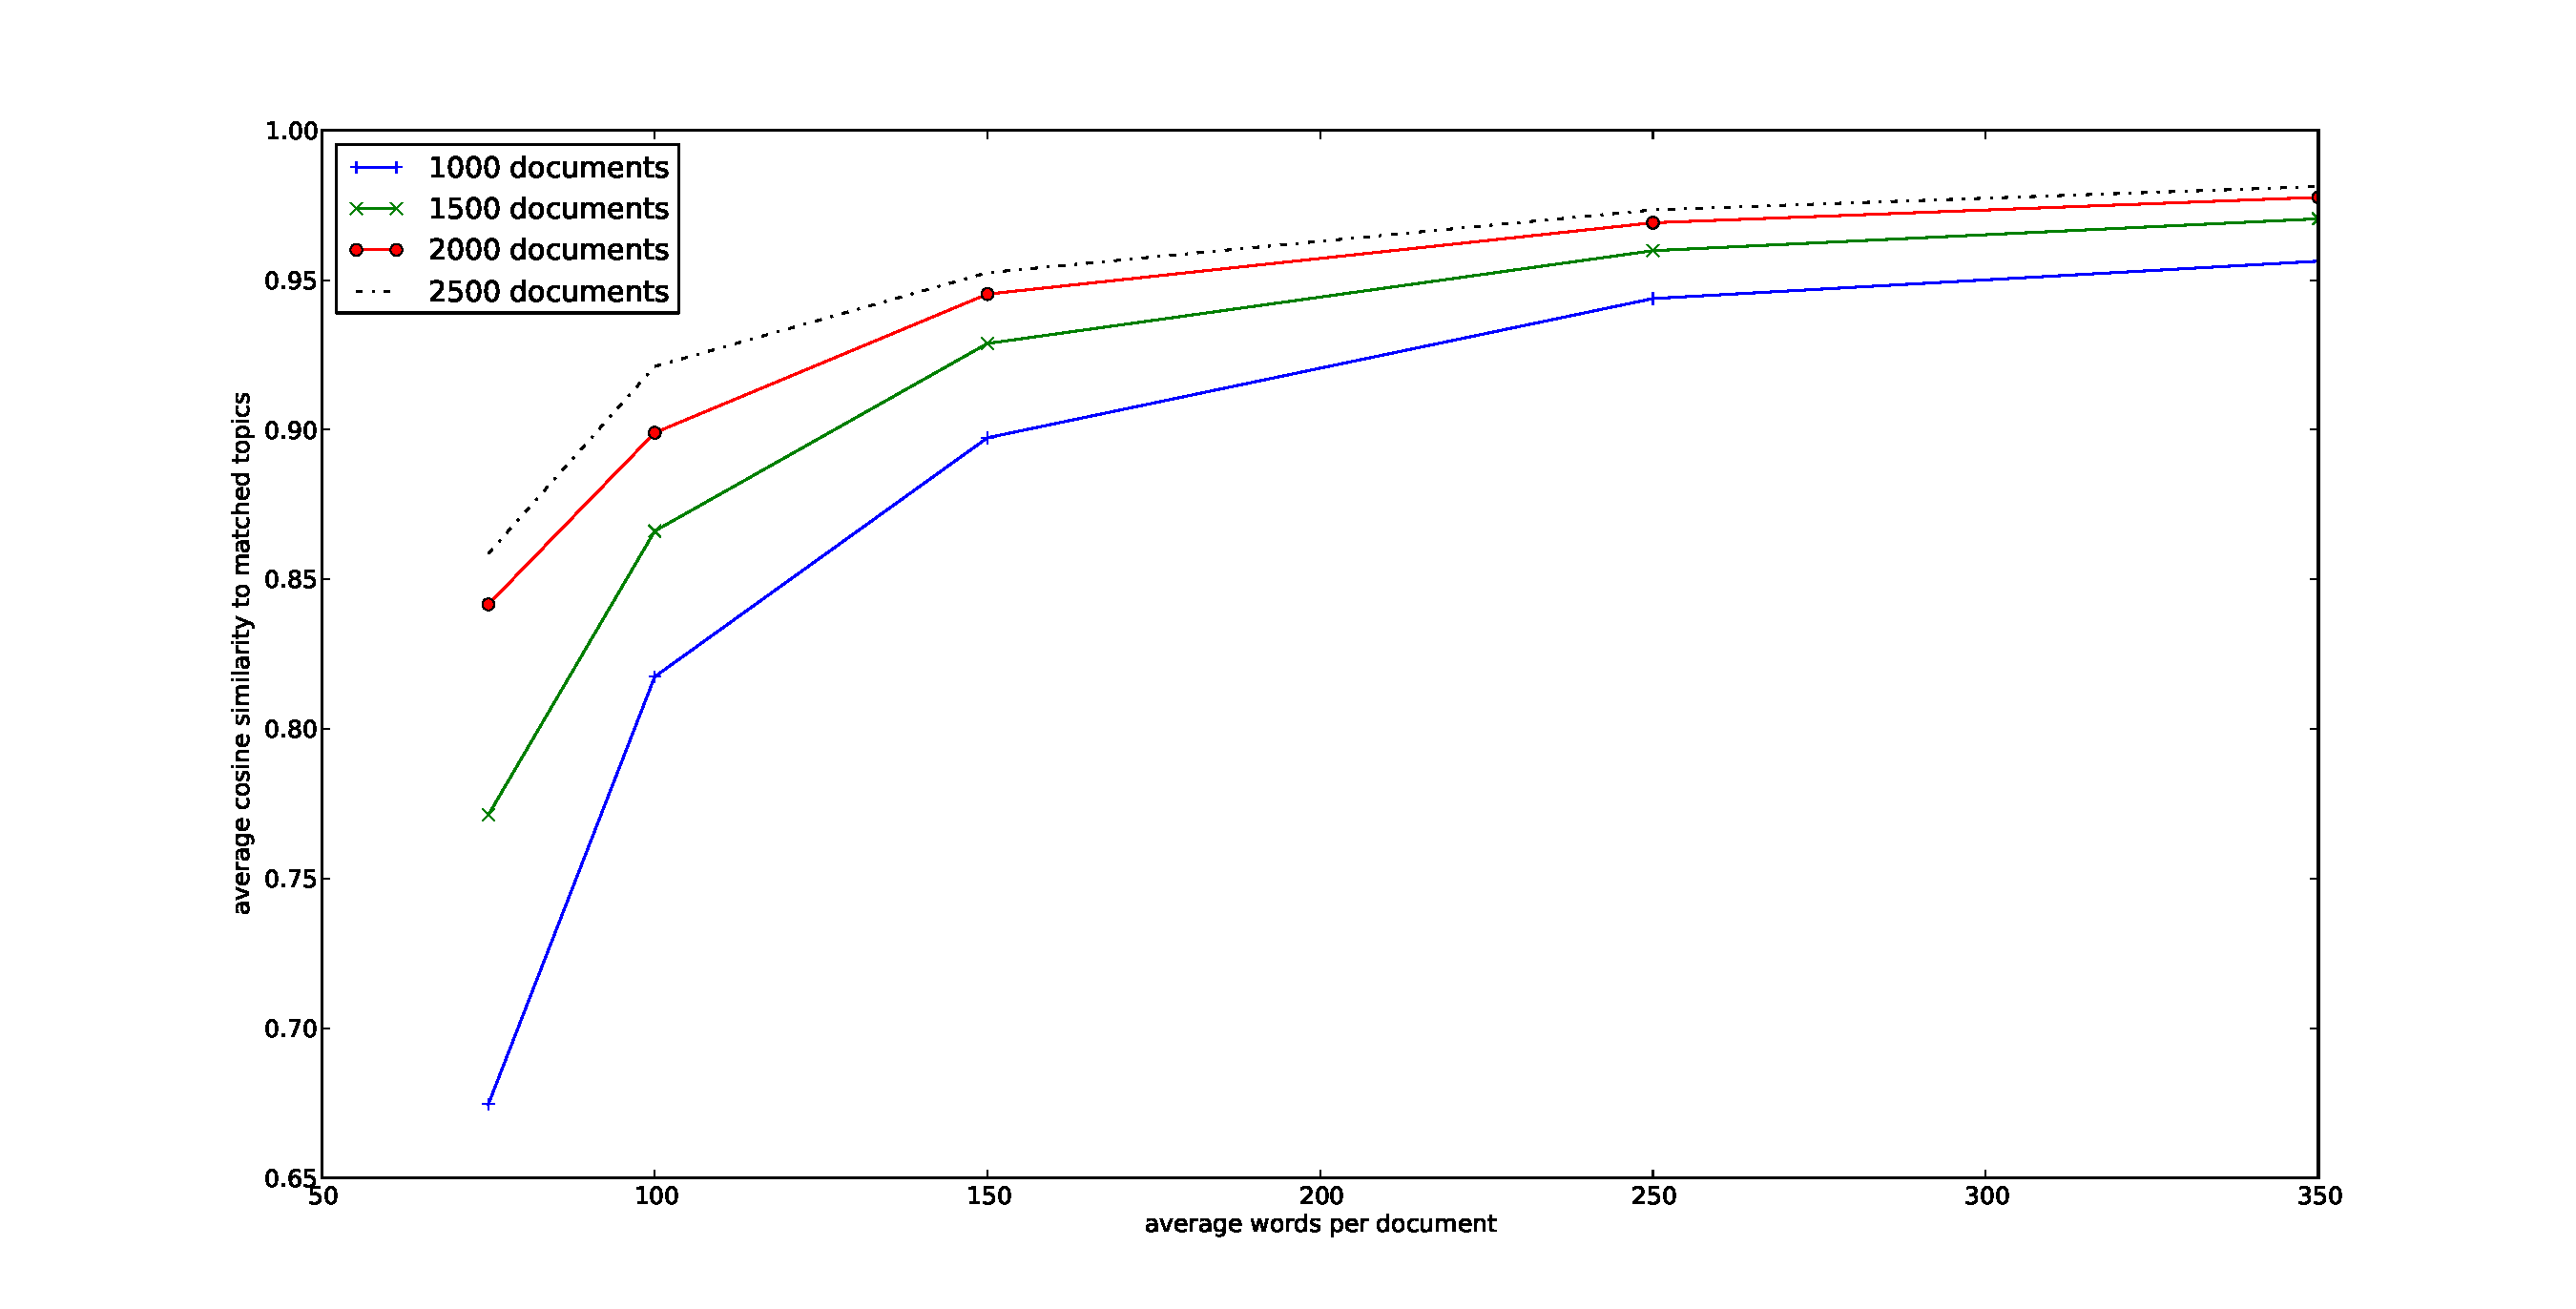
\includegraphics[width=2.5in]{projectorTopics-docs.pdf}
        }
        \subfigure[]{
            \label{fig:b}
            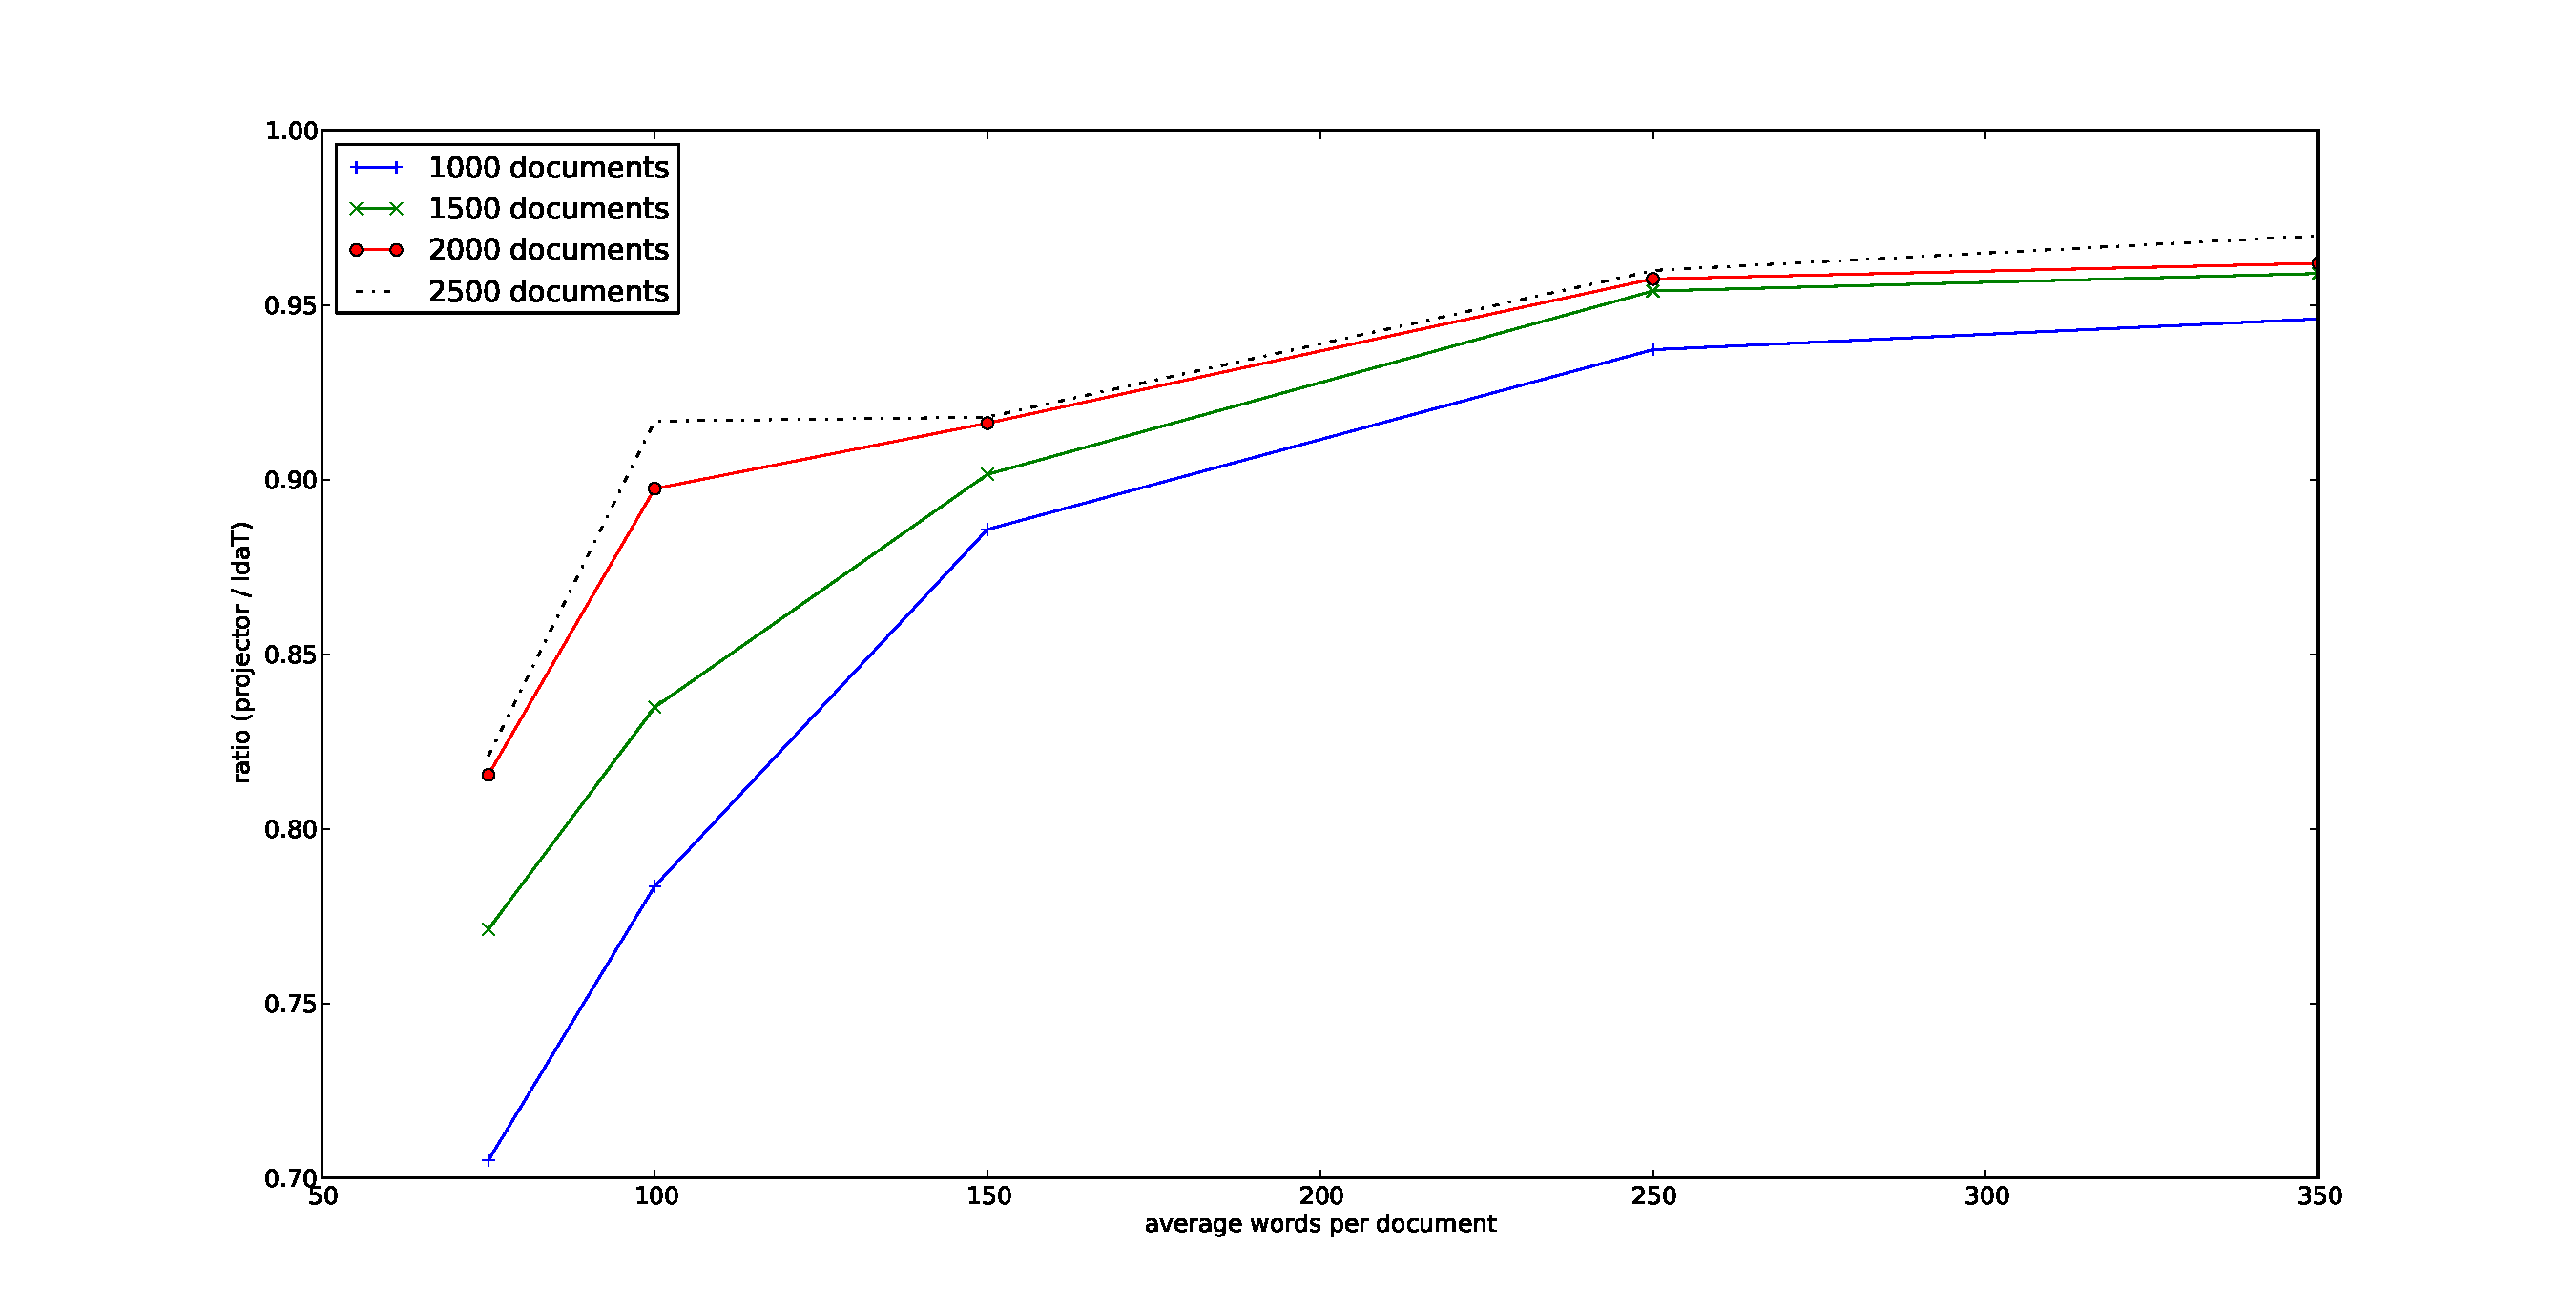
\includegraphics[width=2.5in]{projectorldaT-ratio-docs.pdf}
        }


    \end{center}
    \caption{Figure \ref{fig:a} above shows that as documents grow and document lengths grow, the projector algorithm
learns the topics better.  Figure \ref{fig:b} a corresponding increase in prediction performance comparing the LdaT algorithm that has perfect knowledge of the topics.  The different lines correspond to different numbers of documents, and the $x$-axis corresponds to the number of words in the document.}
   \label{fig:size-matters}
\end{figure}

The basic unit for determining the co-occurence values is the
number of word pairs in the corpus. The number of word pairs
grows quadratically with number of words in a document
and linearly with number of document.  This would indicate
that the performance should improve more as document length
grows as compared with document number.  We note that
the pairs inside the document are not independent but
there is an analysis that shows a nonlinear benefit.


\subsection{An external measure.}


For real world data, there is no access, of course, to the parameters
used in the discussion above. We instead use the chi squared measure
on the cooccurence matrix, $W$.  The analysis above is really just an
anlysis of the cooccurence matrix. The Chi Squared measure is defined
as $$\sum_{i,j} \frac{(W_{i,j} - E_{i,j})^2}{E_{i,j}},$$

where $E_{i,j}$ is the expected number of cooccurrences if
documents are generated from a trivial topic model with
a word distribution equal to the marginal distribution
of the data. 


\begin{figure}
     \begin{center}
            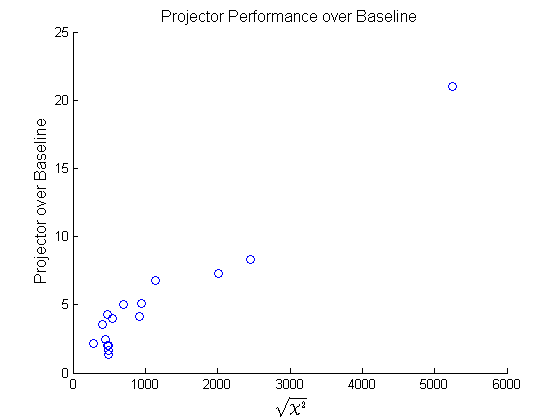
\includegraphics[width=0.45\textwidth]{x2.png}

    \end{center}
    \caption{The x-axis is the log of the Chi Squared measure on the co-occurrence matrix for the words that occur with more than average frequency. Performance relative to baseline increases with increasing Chi squared value.}
   \label{fig:x2}
\end{figure}


We remove all words for the corpus that occur infrequently and
compute the Chi-squared measure on the corresponding co-occurrence
matrix.  In figure~\ref{fig:x2}, we see that this measure 
gives us reasonable insight on the generated data
into when we get good performance on the prediction
task. 


